\documentclass{article}
\usepackage{graphicx}                              %for PNG images (pdflatex)
\usepackage[linkbordercolor={1.0 1.0 0.0}]{hyperref} %for \url tag
\usepackage{color}                                 %for defining custom colors
\usepackage{framed}                                %for shaded and framed paragraphs
\usepackage{textcomp}                              %for various symbols, e.g. Registered Mark
\usepackage{geometry}                              %for defining page size
\usepackage{longtable}                             %for breaking tables
\usepackage{caption}
%
\geometry{verbose,a4paper,tmargin=2.5cm,bmargin=2.5cm,lmargin=2.5cm,rmargin=2cm}
\hypersetup{
  pdfauthor = {Ivan Marton, Peter Stefan},
  pdftitle = {The ARC gLite Gateway},
  pdfsubject = {ARC gLite gateway manual},
  pdfkeywords = {cream2, ARC1, Advanced Resource Connector, manual, users's manual, developers guide, gateway, gLite},
  pdfcreator = {PDFLaTeX with hyperref package},
  pdfproducer = {PDFLaTeX}
}
\bibliographystyle{IEEEtran}                       %a nice bibliography style
\def\efill{\hfill\nopagebreak}
\hyphenation{Nordu-Grid}
\setlength{\parindent}{0pt}
\setlength{\FrameRule}{1pt}
\setlength{\FrameSep}{8pt}
\addtolength{\parskip}{5pt}
%\renewcommand{\thefootnote}{\fnsymbol{footnote}}
\renewcommand{\arraystretch}{1.3}
\newcommand{\dothis}{\colorbox{shadecolor}}
\newcommand{\globus}{Globus Toolkit\textsuperscript{\textregistered}~2~}
\newcommand{\GT}{Globus Toolkit\textsuperscript{\textregistered}}
\newcommand{\ngdl}{\url{http://ftp.nordugrid.org/download}~}
\definecolor{shadecolor}{rgb}{1,1,0.6}
\definecolor{salmon}{rgb}{1,0.9,1}
\definecolor{bordeaux}{rgb}{0.75,0.,0.}
\definecolor{cyan}{rgb}{0,1,1}

\def\documenttitle{The ARC gLite Gateway}
\captionsetup{margin=20pt,font={footnotesize, it},labelfont=bf}
\begin{document}
\def\today{\number\day/\number\month/\number\year}
\begin{titlepage}

\begin{tabular}{rl}
\resizebox*{3cm}{!}{
\includegraphics{logo-knowarc.png}}
\end{tabular}

\hrulefill

%-------- Change this to Knowarc_D<w>.<d>-<n>_<yy>

{\raggedleft Knowarc\_D3.2-1\_08\par}

{\raggedleft \today\par}

\vspace*{2cm}

%%%%---- The title ----
{\centering \textsc{\Large \documenttitle}\Large \par}
%\vspace*{0.5cm}
%%%%---- A subtitle, if necessary ----
%{\centering \textit{\large Paper subtitle}\large \par}
\vspace*{1.5cm}
%%%%---- A list of authors ----
{\centering \large Ivan Marton\footnote{martoni@niif.hu} \large \par}
{\centering \large Peter Stefan\footnote{stefan@niif.hu} \large \par}
%%%%---- An abstract - if style is article ----
%\begin{abstract}
%The abstract
%\end{abstract}
\end{titlepage}
\tableofcontents
\newpage
\section{Introduction}
\label{Introduction}
The purpose of this document is to describe how Advanced Resource Connector version 1 (ARC1\footnote{\url{http://www.nordugrid.org/}}) users can execute grid jobs on EGEE CREAM2\footnote{\url{http://grid.pd.infn.it/cream/}} resources.\par In sections \ref{Introduction} and \ref{Interoperability} a brief introduction on interoperability issues will be given. Section \ref{Building} describes how to build the gateway library, section \ref{Users guide} shows how it can be used. Section \ref{Developers notes} gives a tiny developer-oriented introduction on how the gateway library is built up, while section \ref{Outstanding issues} addresses the current issues with the code. Section \ref{Conclusions} concludes the technical document.
\section{Interoperability}
\label{Interoperability}
Interoperability has been one of the most important disciplines in recent grid middleware development. This term is often used in the sense of accessing resources operated by one kind of grid middleware (e.g. gLite) from a user interface operated by another kind (e.g. ARC1). There are two main possibilities to achieve this result:
\begin{itemize}
\item either to use a special infrastructure element, the gateway, which performs a full data structure and protocol translation between the two inter-operating grid middleware solutions,
\item or to use standard or close-to-standard interfaces on both sides.
\end{itemize}
The latter solution which is preferred from standardization point of view and also has been chosen by ARC1 developers is illustrated in figure \ref{fig:Chart 1}.\par
\begin{figure}[ht]
\centering{\resizebox{\textwidth}{!}{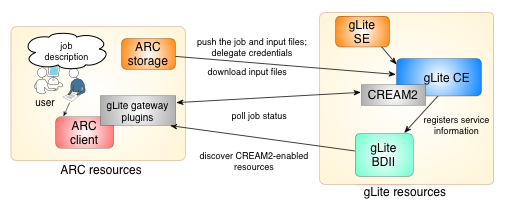
\includegraphics{D3-2-1-figure.png}}
\caption{\label{fig:Chart 1}This chart illustrates how the ARC1$\rightarrow$gLite gateway library works in general. After successful authentication and credential delegation to the CREAM2 resource, users submit grid jobs through it.  A wrapper script at the computing element may pull input files from different storage elements using storage protocol, say, GridFTP. Users get job information through CREAM2 and may send management commands, like kill a job or undelegate credentials.} }
\end{figure}
\section{CREAM2}
The main purpose of this project was to provide access to gLite CREAM2-enabled resources from ARC1 user interface, but not the other way around: i.e. accessing ARC resources from gLite is addressed in the EGEE project\footnote{\url{http://www.eu-egee.org/}}.\par
CREAM2 was chosen for the following reasons:
\begin{itemize}
\item It is a web service interface that fits to the built-in web service implementation of ARC1.
\item It contains numerous improvements compared to the original CREAM interface. (Unfortunately CREAM2 is not backwards compatible with CREAM.)
\item It supports job status queries compared to the other web service interfaces of gLite, like WMProxy.
\item It is an official interface to gLite computing elements and as EGEE evolves it is expected that more and more computing elements will have CREAM2 interfaces.
\end{itemize}
\section{Building, dependencies}
\label{Building}
The ARC$\rightarrow$gLite gateway software is incorporated into ARC1 releases, so you only need to download either the freshest ARC1 from the source tree\footnote{\url{http://svn.nordugrid.org/}} and compile it or to install it from package\footnote{\url{http://download.nordugrid.org/software/nordugrid-arc1/}}.\par
The gateway library code has two dependencies:
\begin{itemize}
\item Globus Toolkit is needed to enable GridFTP functionality to be able to upload input files from the user interface to the CREAM computing node.
\item VOMS is needed to allow users authentication on a CREAM resource.
\end{itemize}
In both cases it is highly recommended to download these pieces of software along with their NorduGrid-specific Globus\footnote{\url{http://download.nordugrid.org/software/globus/}} and VOMS\footnote{\url{http://download.nordugrid.org/software/voms/}} patches from the NorduGrid repository. In case you are interested in the details of patching, then consult the NorduGrid wiki page\footnote{\url{http://wiki.nordugrid.org/images/4/46/NorduGrid-globus.patch.txt}}. It might also be interesting to read how to compile Globus Toolkit. Some more details on this topic can be found on the NorduGrid Globus compilation page\footnote{\url{http://wiki.nordugrid.org/index.php/Globus\_Libraries}}. There are also some details on how to compile VOMS from source at NorduGrid VOMS compilation page\footnote{\url{http://wiki.nordugrid.org/index.php/VOMS\_compiling\_detailes}}.
\section{Using the ARC${\rightarrow}$gLite Gateway from the Command Line}
\label{Users guide}
There are seven different command line tools for using the gLite gateway functions. In this section these tools will be presented in detail through examples. The job descriptions and services shown are just simple examples, they might be different in real-life usage.\par
Every tool has a short manual page being accessible by using the \textbf{man} on-line manual reader command or some more help can be achieved by using the $<$command$>$ -? command line option.\par
Before getting into the details of the gatewy toolkit, the authentication and authorization processes need clarification.\par
In the different grid systems the most widespread authentication method is the certificate based authentication. GLite also requires VOMS-enabled proxy X509 certificates to access resources. It means that you should be a member of the Virtual Organisation that is valid on the remote site. If the VOMS package has been correctly installed then the following command provides the necessary VOMS proxy certificate.\par
\begin{shaded}\verb#$ voms-proxy-init -voms <Your Virtual Organisation>#\end{shaded}
For example:
\begin{shaded}\verb#$ voms-proxy-init -voms knowarc.eu#\end{shaded}
CREAM2 service URLs can directly be downloaded from any BDII database of gLite using the following LDAP command:
\begin{shaded}
\verb#$ ldapsearch -x -h lcg-bdii.cern.ch -p 2170 -b o=grid '(GlueCEUniqueID=*blah*)'#
\end{shaded}
or
\begin{shaded}
\verb#$ ldapsearch -x -h lxbra2305.cern.ch -p 2170 -b mds-vo-name=local,o=grid //#\\*
\verb#        '(GlueCEUniqueID=*cream*)' | grep GlueCEInfoContactString | //#\\*
\verb#        awk '{print $2}' | sort | uniq#
\end{shaded}

\subsection{glitedelegate}
\label{glitedelegate}
If you want to submit a job to a gLite server, first you have to own a valid delegation on the remote site. You can either use an old, but still valid delegation identifier, or register a new one. There is a command line tool to register a delegation on the resource to be used.\par
The usage is very easy and straighforward. All you need is a working CREAM2 service URL, and a locally unique arbitrary delegation ID. This delegation ID will be associated to the remote resource. If you are not sure wether your favourite delegation ID is occupied or not, then try to delete it before registering it again. (See Section \ref{gliteundelegate} for further details!) The delegation command has the following syntax:
\begin{shaded}\verb#$ glitedelegate <delegation ID> <service URL>#\end{shaded}
For example:
\begin{shaded}\verb#$ glitedelegate test_delegation //#\\*
\verb#        https://cream.grid.upjs.sk:8443/ce-cream/services/gridsite-delegation#\end{shaded}
\subsection{glitesub}
\label{glitesub}
In the previous section it was shown how to create delegation. (See Section \ref{glitedelegate}!) This function, the job submission, is the only one which needs the delegation ID.\par The next step is to prepare the necessary input files and the job description!\par
The glitesub command syntax is the following:
\begin{shaded}\verb#$ glitesub -D <delegation ID> <service URL> <job description> <info file>#\end{shaded}
Here the delegation ID is the previously registered identification. The service URL will be different than in the delegation example above, because this is not the URL of the delegation, but the execution service. The job description must be in JDL format like in the example below. The info file stores information about job submitted. It should either be a non-existing file or it is overwritten. This file contains the job ID, the input sandbox URL, the output sandbox URL and the service URL. The submission command will take care of uploading the necessary input files up to the execution node.\par
It is important that the \textit{VirtualOrganisation} and \textit{QueueName} attributes should be the same as your virtual organisation name and the corresponding queue name on the server side.\par

An example JDL description:\\
\begin{minipage}{\textwidth}
\begin{framed}
\verb#[#\\
\verb#Executable = "/bin/hostname";#\\
\verb#StdInput = "std.in";#\\
\verb#StdOutput = "std.out";#\\
\verb#StdError = "std.err";#\\
\verb#BatchSystem = "pbs";#\\
\verb#VirtualOrganisation = "knowarc.eu";#\\
\verb#InputSandbox = {"std.in"};#\\
\verb#OutputSandbox = {"std.out","std.err"};#\\
\verb#QueueName = "knowarc.eu";#\\
\verb#OutputSandboxDestURI = { "gsiftp://localhost/std.out", "gsiftp://localhost/std.err" };#\\
\verb#]#
\end{framed}
\end{minipage}
An example how to use this command:
\begin{shaded}\verb#$ glitesub -D test_delegation //#\\*
\verb#        https://cream.grid.upjs.sk:8443/ce-cream/services/CREAM2 description.jdl job.info#\end{shaded}
\subsection{glitestat}
\label{glitestat}
The \textbf{glitestat} tool extracts job information about a CREAM2 job identified by the information file. This file made by command \textbf{glitesub} is the only argument needed here.\par
Usage:
\begin{shaded}\verb#glitestat <info file>#\end{shaded}
For example:
\begin{shaded}\verb#glitestat job.info#\end{shaded}
The possible responses and their meanings are the following:
\begin{itemize}
\item ACCEPTING - The job submission is comleted but the job is not yet scheduled
\item SUBMITTING - Scheduling in progress
\item INLRMS:Q - The job is already at the local resource manager system and it is queued
\item INLRMS:R - The job is waiting at the local resource manager system for running
\item INLRMS:S - The job is actually running
\item KILLED - The job was terminated
\item FINISHED - The job has finished
\item FAILED - The job had some failure
\item FAILES - The job had some failure at LRMS level
\item EXECUTED - The job has been finished and there is no stating information available
\end{itemize}
\subsection{glitekill}
\label{glitekill}
The \textbf{glitekill} command can be used for killing a remote job. The only necessary argument is the information file made by \textbf{glitesub}. (See Section \ref{glitesub} for further details!) This command initiates stopping the job. You can check the effect by using \textbf{glitestat}. (See Section \ref{glitestat} for its usage!)\par
Usage:
\begin{shaded}\verb#glitekill <info file>#\end{shaded}
For example:
\begin{shaded}\verb#glitekill job.info#\end{shaded}
\subsection{gliteclean}
\label{gliteclean}
Either after killing a job or because of some remote error occurs garbage files may remain on the server. These files can be purged by using command \textbf{gliteclean}. If you intentionally kill a job on the computing node, the job related stuff might also remain as garbage in the remote queue. This command also removes the job from the gLite server queue. It is important to note that this command removes the local information file as well. It is very useful to run this command after killing a job. (See Section \ref{glitekill}!)\par
Usage:
\begin{shaded}\verb#gliteclean <info file>#\end{shaded}
For example:
\begin{shaded}\verb#gliteclean job.info#\end{shaded}
\subsection{gliteundelegate}
\label{gliteundelegate}
After your work is complete it is possible to unregister and delete the delegation entry from the remote site by using command \textbf{gliteundelegate}. You can also use it, if you want to register a delegation ID but are unsure whether it is used or not. Put the delegation service URL into the argument!\par
Usage:
\begin{shaded}\verb#$ gliteundelegate <delegation ID> <service URL>#\end{shaded}
For example:
\begin{shaded}\verb#$ gliteundelegate test_delegation //#\\*
\verb#        https://cream.grid.upjs.sk:8443/ce-cream/services/gridsite-delegation#\end{shaded}
\section{Developers notes}
\label{Developers notes}
This section describes how to use the library on your own client. The base class of the gLite client is written as an ARC Client Component (ACC) but also can be used as a standalone library. There is nothing more to be done just to link the \textbf{CREAMClient}, \textbf{arcclient} and \textbf{arccommon} libraries installed with the ARC1 sofware and to create an instance of the \textit{CREAMClient} class.\par
This client object has a very easy-to-use and intuitive interface. It uses the VOMS proxy certificate to build the secure channel to the server and to sign that of the server's. Actually the client looks for this certificate just at its default location. If you want to store it somewhere else, you have to modify the source code itself.\par
The different functions throw \textit{CREAMClientError} exceptions that should be caught in the application.\par
The following sections present the set of functions provided by the library.
\subsection{CREAMClient(Arc::URL, Arc::MCCConfig)}
The constructor of the class performs the necessary initialization work. It receives two arguments: the service URL and the ARC message chain component configuration file to establish the communication channel to the server. These pieces of information are indispensable to create your client and to communicate with the remote site.
\subsection{setDelegationId(std::string)}
Besides the constructor this is the other generic-purpose function that can be used in CREAM2 client applications. This function sets the previously registered and referred delegation ID on the client. The function is very simple: just set a private variable and returns with no value.
\subsection{createDelegation(std::string)}
The \textbf{createDelegation} function is about to perform the whole delegation registration process. It sends a \textit{getProxyReq} message having the requested delegation ID, signs the received certificate and sends it back in a \textit{putProxy} SOAP message to the server. These three steps constitute the delegation registration process.
As almost every funtion, this one has no return value either. If there are any problems during the communication, either locally in the channel or at the remote site, the function throws \textit{CREAMClientError} described previously. If there are no exceptions thrown, then the command is considered to have been successfully completed.
\subsection{destroyDelegation(std::string)}
This method has the reverse functionality of the \textbf{createDelegation} function. It sends the CREAM2 \textit{destroy} message to the remote server.
\subsection{submit(std::string)}
The \textbf{submit} function is the most complex part of the class. It translates the job description received as the argument, registers the job with a \textit{JobRegisterRequest} message, uploads the locally stored files, if necessary, then enables the job execution on the server by sending a \textit{JobStartRequest} message. Finally it returns with a \textbf{creamJobInfo} object that contains a \textit{jobId} (job indetifier), a \textit{creamURL} (as the service URL), an \textit{ISB} (reference to the Input Sandbox) and an \textit{OSB} (Output Sandbox) member to describe the registered job. In the \textbf{glitesub} command (See Section \ref{glitesub} for details) these pieces of information are stored in the information file.
\subsection{stat(std::string)}
This method queries the job status from the gLite CREAM2 server. The return value is the job status translated to the ARC terminology. The possible values are presented in the section of the \textbf{glitestat} command line tool. (See Section \ref{glitestat}!)
\subsection{cancel(std::string)}
The \textbf{cancel} function sends a \textit{JobCancelRequest} SOAP message to the server and handles the emerging exceptions. It can be used for canceling a remotely registered and possibly running job.
\subsection{purge(std::string)}
The \textbf{purge} function sends a \textit{JobPurgeRequest} message to server and throws an exception in case of any emerging problems.
\subsection{An example gLite client}
Finally, here is an example code to present how easy and simple is to write a new client. This code sample requests the job status of a previously submitted remote job, and writes it to the standard output. The client is written in C++.
\begin{framed}
\verb?#include "CREAMClient.h"?\\*
\verb?#include <iostream>?\\*
\\*
\verb?int main(int argc, char* argv[]){?\\*
\verb?  Arc::URL url( SERVICE_URL );?\\*
\verb?  Arc::MCCConfig cfg;?\\*
\\*
\verb?    Arc::Cream::CREAMClient gLiteClient(url,cfg);?\\*
\verb?    try {?\\*
\verb?        std::cout << "Job status: " << gLiteClient.stat( JOBID ) << std::endl;?\\*
\verb?    } catch (CREAMClienException& cce) {?\\*
\verb?        std::cerr << "ERROR: " << cce.what() << std::endl;?\\*
\verb?        return 1;?\\*
\verb?    }?\\*
\verb?    return 0;?\\*
\verb?}?
\end{framed}
It is of course mandatory to define \textit{SERVICE\_URL} and \textit{JOBID} strings to their real values to reach the proper functionality.
\section{Outstanding issues}
\label{Outstanding issues}
Even though the gateway library code is ready for production use, there are a couple of issues to be handled in the upcoming development.
\subsection{Full ARC1 client integration}
Full ARC1 client integration basically means that the previously presented commands will disappear and their functionality will be available in the standard ARC1 client toolkit. However there are two dependencies to be met to achieve this stage:
\begin{itemize}
\item On one hand ARC1 broker along with the BDII-capable target object should be finalized.
\item On the other hand a conflicting Globus Toolkit OpenSSL and the standard OpenSSL issue is to be investigated.
\end{itemize}
The latter issue was revealed when the VOMS proxy certificate delegation method was implemented in the gateway library. Since in the ARC1 client-side library there is a built-in Message Chaining Component (MCC) which already uses Globus Toolkit OpenSSL functions to enable establishing secure communication. Linking glite* tools directly against the standard OpenSSL libs caused congesting SSL functions which led to the breakdown of the whole library. The solution had been not linking the standard OpenSSL libs, just the patched OpenSSL in the Globus Toolkit.
\subsection{xRSL${\rightarrow}$JDL translation and related problems}
It is possible to express jobs in XRSL which have no equivalent in JDL. Specifically, in XRSL it is possible for input files downloaded from storage servers to have their names changed. This is not possible in JDL. So a user might in XRSL ask for this:
\begin{shaded}
\verb#(inputfiles=(gsiftp://interop.dcgc.dk/storage/datafile1.txtinput.txt))#
\end{shaded}
That is not possible to express in JDL. It only allows the file to be downloaded as datafile1.txt. This could be solved by a wrapper script that renames files according to the XRSL specification. This does not solve our problem completely however. For example if a user wants to concatenate the stdout from two jobs, he would write something like the following in XRSL:
\begin{shaded}
\verb#(inputfiles=(gsiftp://interop.dcgc.dk/storage/job1/output.txtinput1.txt)#\\*
\verb#            (gsiftp://interop.dcgc.dk/storage/job2/output.txtinput2.txt))#
\end{shaded}
This cannot be solved just using the renaming method, because both input files would be retrieved before renaming is done and they would therefore overwrite each other.\par
The solution is to recognize jobs of this type and simply barring them from using gLite resources or to let such jobs fail with an error message explaining that the user has to express their job in a different way.
\subsection{RunTime Environments related issues}
Many grid jobs rely on software being available at the execution location. The requirement as well as the initialization 
of such software is expressed through the use of Run-Time Environments (RTEs). While the library is capable of 
translating the RTE request itself it is not capable of translating the name of the RTE. No standardized cross Grid 
nomenclature has been adopted, nor are the authors aware of any such activity. A temporary solution would be for each 
VO to have a remotely accessible list of RTEs and their names in each job description language. This could then be used for translating jobs.
\section{Conclusions}
\label{Conclusions}
The document has described an ARC1 library extension that allows ARC1 grid users to access gLite CREAM2 computing resources. The current version of the code allows direct access to resources but as the new ARC1 brokering solution comes out the gateway functionality will be integrated fully into the ARC1 client code. The same version will also be able to access the gLite information system to extract CREAM2 resource information.\par
A built-in xRSL${\rightarrow}$JDL translator will also enable to use purely xRSL job description on ARC1 user interfaces.
\end{document}
